\chapter{Experiment Apparatus}
\label{experiment}

All data used in the analysis described in this thesis was produced by high energy $\ppbar$ collisions at the Tevatron $\ppbar$ accelerator and recorded by the $\dzero$~detector. The Tevatron is currently the only collider in the world with enough center of mass energy to directly produce top quarks in relative abundance. Section.~\ref{tevatron} describes how protons are accelerated to an energy of 980 GeV as well as how antiprotons are created to produce $\ppbar$~collisions at a center of mass energy of $1.96$~TeV. Sections~\ref{ppbarcollisions} and~\ref{coordinate} give an introduction to $\ppbar$~collisions and useful quantities used to described particles produced in the collisions. Finally, Section~\ref{detector} describes the $\dzero$~detector that is used to collection information about the particles produced in the $\ppbar$~collisions. 

\section{Fermilab Accelerator Complex}
\label{tevatron}

The Fermilab accelerator complex is a chain of accelerators designed to produce and collide two circulating beams of protons and antiprotons each with an energy of 980 GeV. Five unique accelerators are employed to create and accelerate protons and antiprotons. The five accelerators, described in more detail in this section, are the Cockcroft-Walton, the LINAC, the Booster, the Main Injector, and the Tevatron Main Ring. Fig.~\ref{Tevatron} shows a schematic of these accelerators.

%\begin{figure}[!h!tbp]
%\begin{center}
%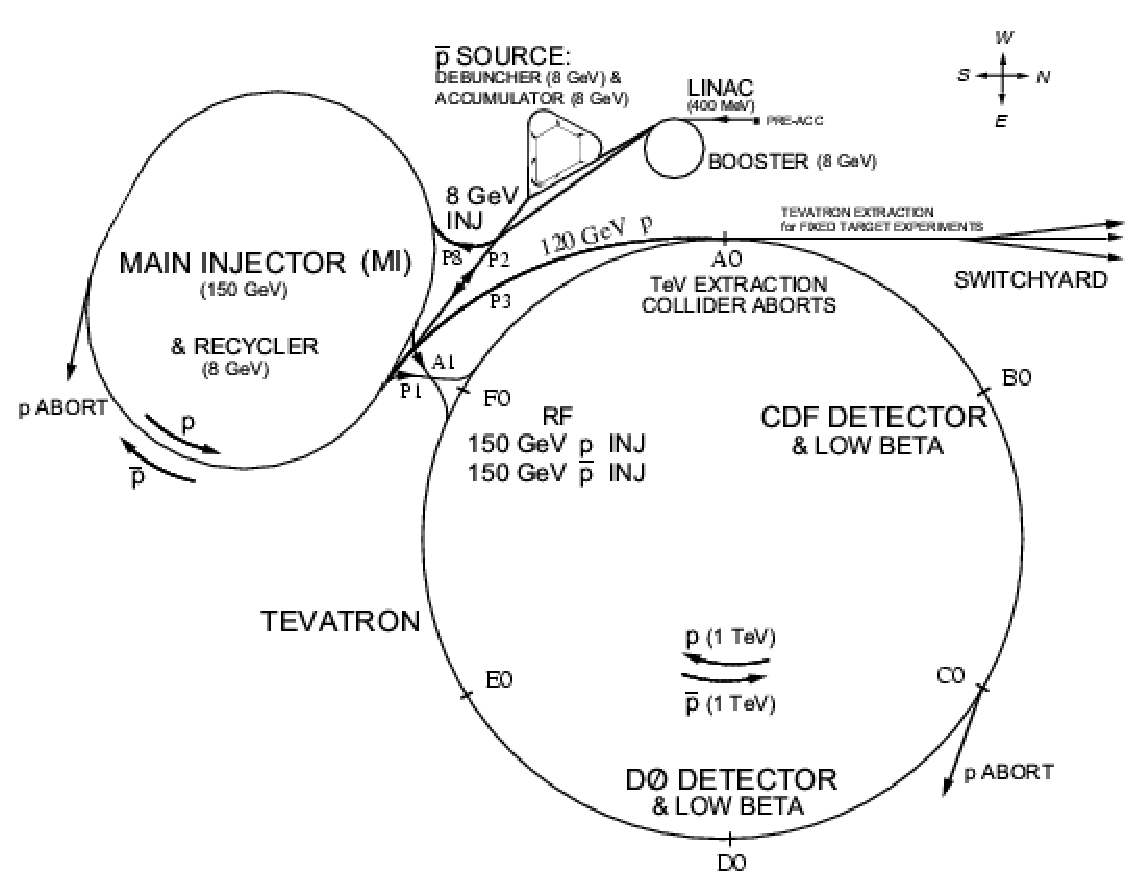
\includegraphics[width=0.75\textwidth]{eps/Tevatron/Tevatron.eps}
%\end{center}
%\vspace{-0.1in}
%\caption{Fermilab Accelerator Chain}
%\label{Tevatron}
%\end{figure}


\subsection{Cockcroft-Walton}
The first accelerator in the chain is the Crockroft-Walton. In this accelerator, a hydrogen gas is heated in a plasma which allows an additional electron to bond with the hydrogen atom producing a net negative charge. The Crockroft-Walton is a DC voltage ladder that produces a voltage difference of 750~kV across which the newly negatively hydrogen ions are accelerated.

\subsection{LINAC}
After the negatively charged hydrogen ions have been accelerated to an energy of 750keV, they are further accelerated by the LINAC (LINear ACcelerator). The LINAC is a 130-m long set of metallic tubes separated by vacuum gaps. An alternating electric field produced by a radio frequency (RF) power source accelerates the negatively charged hydrogen ions across the gap while the field is electric field is parallel with the ion direction of motion. When the field direction reverses the ions are shielded by the metallic tubes. As the ions increase their speed the gap length and drift tube length increases as shown in Fig.~\ref{LINAC}. Because the LINAC uses an alternating electric field the continuous ion beam produced by the Crockoft-Walton is altered such that the protons are concentrated (``bunched") together. By the end of the acceleration the proton bunches are separated by 5 ns and have an energy of 400 MeV. The final step in the LINAC is to remove the orbital electrons by passing the ions through a carbon foil leaving only the positively charged protons.

\begin{figure}[!h!tbp]
\begin{center}
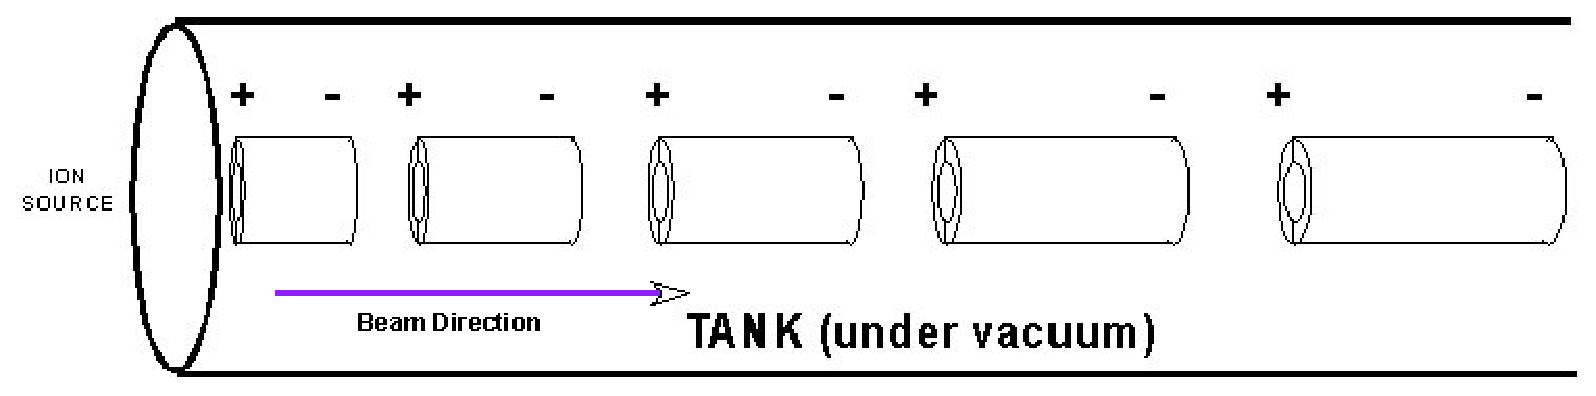
\includegraphics[width=0.75\textwidth]{eps/Tevatron/LINAC.eps}
\end{center}
\vspace{-0.1in}
\caption{Cartoon example of the linear accelerator's alternating series of gaps and drift chambers.}
\label{LINAC}
\end{figure}

\subsection{Booster}
The next accelerator in the chain is the Booster, which is a circular synchrotron accelerator 475-m in circumference. The Booster consists of RF cavities that accelerate the 400 MeV proton bunches to an energy of 8 GeV. The proton bunches circulate the Booster 16,000 times and the entire acceleration process takes 33 ms.

\subsection{Main Injector}
The Main Injector is the next accelerator in chain after the Booster. The Main Injector also uses RF cavities to accelerate the proton bunches to an energy of 120 GeV and employs strong magnets to keep the protons along a circular path. After the acceleration, there are two possible paths for the protons: $\bar{p}$~production or continued acceleration. The protons that will eventually circulate in the Tevatron ring are further accelerated to an energy of 150 GeV and then continue to circulate the Main Injector ring until needed. The remaining protons are used to create antiprotons that will also eventually circulate in the Tevatron ring. Antiprotons are created when 120 GeV protons from the Main Injector strike a fixed 7 cm thick nickel target producing a spray of short lived particles and anti-particles. From this spray roughly 20 antiprotons are produced for every million protons used. All particles produced from the collision are focused and collimated by use of a lithium lens. To separate the antiprotons from the other particles, a bending magnet is employed to remove all positively charged particles as well as particles with masses different from the proton mass. To remove the remnant bunch structure, the antiprotons are passed through a debuncher, which separates the antiprotons in space-time as well as reducing the energy spread. To further reduce the energy spread of the antiprotons, a process called stochastic cooling is applied. This process uses ultra-cold electronics (-$452^{\circ}$~F) to detect and alter particles trajectories to make their orbits and thereby their energies more uniform. Because each $\ppbar$~collision requires $\sim10^{10}$ antiprotons, the final stage for $\bar{p}$~production is to collect and store large quantities of antiprotons. This is done with the accumulator, which allows for many circulating beams of antiprotons to be kept for many hours. Once enough antiprotons have been collected, they are sent to the Main Injector where they are accelerated to a final energy of 150 GeV. At this stage the antiprotons circulate clockwise and the protons circulate counter-clockwise in the single ring of the Main Injector.

\subsection{Tevatron Main Ring}
The final stage of the acceleration process is a superconducting accelerator called the Tevatron. The Tevatron accelerates protons and antiprotons to an energy of 980 GeV using RF cavities in the same manner as the Booster and the Main Injector. The Tevatron uses nearly 1,000 superconducting magnets running at $4.3^{\circ}$~K with a magnetic field strength of $4.2$~T to bend the two circulating beams around the nearly 6~$\frac{1}{2}$ km circumference. At an energy of 980 GeV, the bunches circulate the Tevatron ring nearly 57,000 times per second and cross one-another every 396 ns. The two circulating beams are kept far enough apart in the ring to avoid direct collisions unless they are further focused. In the Tevatron ring there are two places where the beams are focused, which correspond to the two large experiments: $\dzero$ and CDF.


\section{$\ppbar$~Collisions}
\label{ppbarcollisions}

When the two circulating beams at the Tevatron are brought into focus an enormous range of kinematically allowed processes and final state decays are possible. While the outcome of a particular $\ppbar$~collision is random, the rate at which certain processes occur can be calculated with the Standard Model framework. The most common type of collision is an inelastic $\ppbar$~collision which produces one or more particles scattered at low angles with respect to the beam axis. These processes usually do not involve much energy transfer between the colliding particles and are therefore called low-energy or low-$p_{T}$ events. More rare processes, such as top quark or W boson production, require much more energy to be transferred between colliding particles. These processes occur when one of the constituent quarks or gluons inside the proton collide with another quark or gluon from the antiproton. This process is sometimes referred to as the hard-scatter process. The hard-scatter process can produce on-shell resonances ($Q^{2} = M^{2}$) of heavy particles such as W Boson or sometimes it can produce very short lived vritual particles ($Q^{2} \neq M^{2}$) such as the case with $s$-channel single top quark production where a W boson is produced with $Q^{2} > M_{W}^{2}$.

The heavy particles produced in the hard-scatter collision will decay into more stable particles as governed by the interactions allowed in the Standard Model. For very heavy particles with short lifetimes the decay happens in a space much smaller than the resolution of any detector. For instance, the top quark lifetime is $\sim10^{-24}$~s which is many orders of magnitude smaller than the fastest detector electronics. In fact, almost all short-lived particles produced in the hard-scatter can not be measured directly, but instead their presence is inferred from precise measurements of the their decay products. Making precise measurements of these decay products is the chief goal of all high energy detectors.

The remainder of this chapter is dedicated to describing the $\dzero$~detector and how it makes the measurements required to infer the presence of the heavy resonances such as the top quark. Section~\ref{coordinate} describes the coordinate system convention used throughout the rest of the chapter as well as introduces several new units typically used in high energy physics. Section~\ref{detector} describes the $\dzero$~detector and explains how it is used to measure the particles, such as muons or pions, resulting from the $\ppbar$~collisions at the Tevatron.

\section{Coordinate System and Units Convention}
\label{coordinate}

The $\dzero$~detector is usually described using a spherical coordinate system ($r$,$\theta$,$\phi$) with an origin located at the center of the detector. The angle $\theta$ is defined with respect to the beam axis where $0^{\circ}$ is aligned with the proton direction and $180^{\circ}$ is aligned with the antiproton direction. The angle $\phi$ is defined with respect to the $x$-axis as shown in Fig.~\ref{coordinate-eps}. The $z$-axis is defined to be parallel with the beam axis with the positive direction corresponding to $\theta = 0^{\circ}$ and the negative direction corresponding to $\theta = 180^{\circ}$.

\begin{figure}[!h!tbp]
\begin{center}
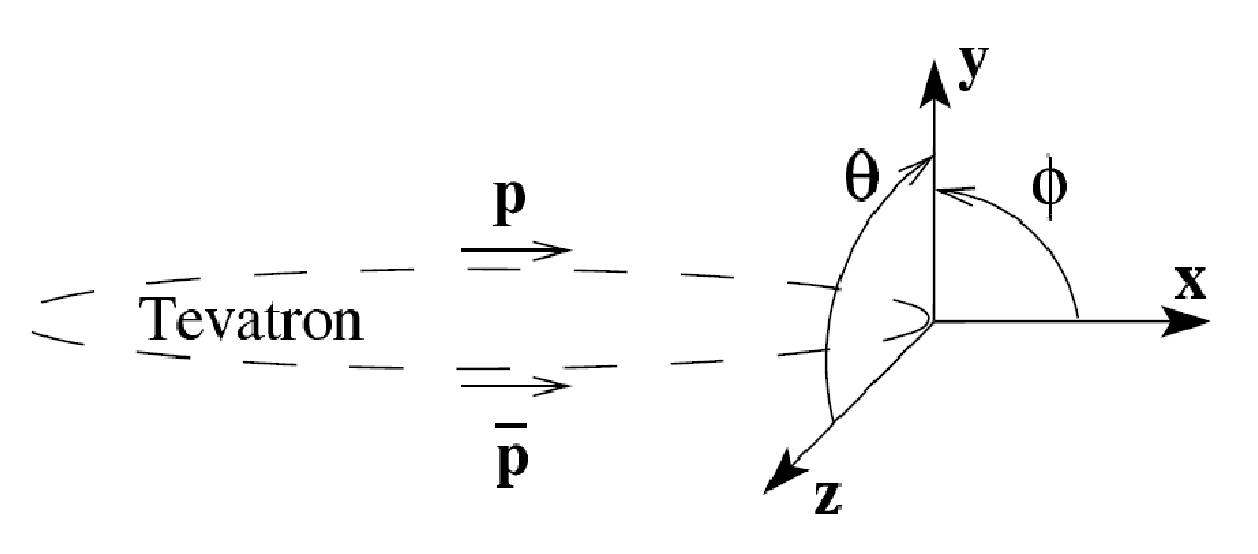
\includegraphics[width=0.75\textwidth]{eps/Tevatron/Coordinate.eps}
\end{center}
\vspace{-0.1in}
\caption{Tevatron coordinate system}
\label{coordinate-eps}
\end{figure}

It often convenient to convert the angle $\theta$ to a quantity called pseudorapidity, $\eta$, defined in Eq.~\ref{pseudorapidity}.

\begin{equation}
\label{pseudorapidity}
\eta = -\ln \left[ \tan \left( \frac{\theta}{2} \right) \right]
\end{equation}

This quantity is identical, in the limit of massless particles, to the true rapidity, $y$ shown in Eq.~\ref{rapidity}, which is invariant under a Lorentz boost along the $z$-direction. This is useful because $\ppbar$~-collisions at the Tevatron can and usually do occur with such a boost. The pseudorapidity is $0$ for a particle with $\theta = 90^{\circ}$ and approaches $\infty$ as $\theta \rightarrow 0^{\circ}$.

\begin{equation}
\label{rapidity}
y = \frac{1}{2}\log \left[ \frac{E + p_{z}}{E - p_{z}} \right]
\end{equation}

Another quantity used when describing the relationship between two objects or the size of an object in the $\dzero$~detector is the solid angle, $\Delta R$, defined in terms of $\Delta\phi=\phi_{1} - \phi_{2}$~and $\Delta\eta=\eta_{1} - \eta_{2}$.

\begin{equation}
\Delta R = \sqrt{(\Delta\phi)^{2} + (\Delta\eta)^{2}}
\end{equation}

Finally, the quantity of luminosity is important when describing the intensity of an interaction or of the accumulated amount of data. The rate of a certain process is equal to the luminosity, $\mathcal{L}$, times the Lorentz invariant cross section, $\sigma$, as shown in Eq.~\ref{rate}.

\begin{equation}
\label{rate}
\rm{Rate} = \frac{dN}{dt} = \sigma * \mathcal{L}
\end{equation}

Most cross sections at the Tevatron are given in terms of pico-barns ($10^{-36}$~cm$^{2}$) and thus the units of luminosity are pb$^{-1}$s$^{-1}$. The integrated luminosity, $\int \mathcal{L} dt$, with units of pb$^{-1}$, is used when discussing total number of events.


\section{\dzero~ Detector}
\label{detector}

The $\dzero$~detector, schematically shown in Fig.~\ref{D0}, is designed to collect as much information as possible from the $\ppbar$~collisions at the Tevatron. The detector is really a collection of smaller sub-detectors that work in tandem to precisely measure all decay products from a hard-scatter collision. The inner-most detectors are the tracking detectors, described in Section~\ref{tracking}, which record the paths of charged particles as they enter and leave the detector. The next layer of the detector is the calorimeter, described in Section~\ref{calorimetry}. The calorimeter measures the energy of the lightest electromagnetically interacting particles, such as the electron and the photon, and strongly interacting particles, such as pions or neutrons. Another sub-detector, called the luminosity monitor, described in Section~\ref{luminositydetector}, records whether or not their was a true inelastic $\ppbar$~collision. The outer-most layer of the $\dzero$~detector is the muon detector, described in Section~\ref{muondetector}. Once the collision has been measured, a complex set of trigger decisions, described in Section~\ref{triggersystem}, must be satisfied before the event is recorded to tape for later reconstruction and analysis.


\begin{figure}[!h!tbp]
\begin{center}
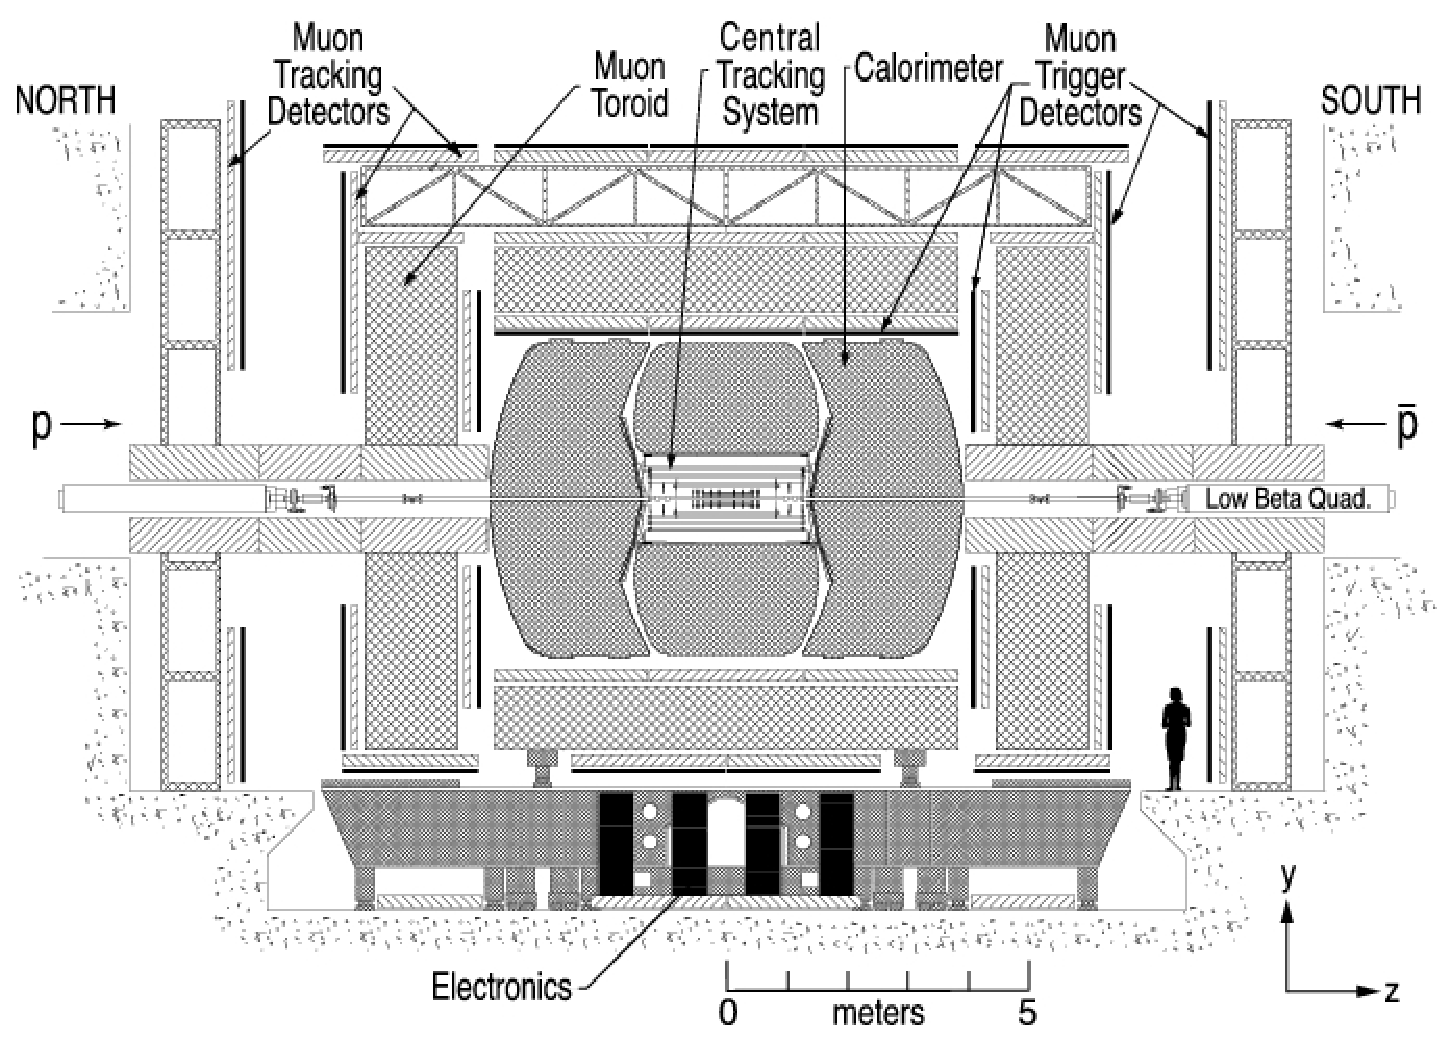
\includegraphics[width=1.0\textwidth]{eps/D0/DetectorSlice2.eps}
\end{center}
\vspace{-0.1in}
\caption{Schematic side-view of the $\dzero$~detector.}
\label{D0}
\end{figure}

\subsection{Tracking Detectors}
\label{tracking}

The innermost layer of the $\dzero$~detector is a set of two tracking detectors designed to measure the flight path of charged particles. The twos detectors, shown in Fig.~\ref{InnerDetector}, are the silicon microstrip tracker (SMT) and the central fiber tracker (CFT). The SMT and CFT are located within a 2T magnetic field generated by a superconducting solenoid magnet. The preshower detectors are located immediately outside the solenoid.


\begin{figure}[!h!tbp]
\begin{center}
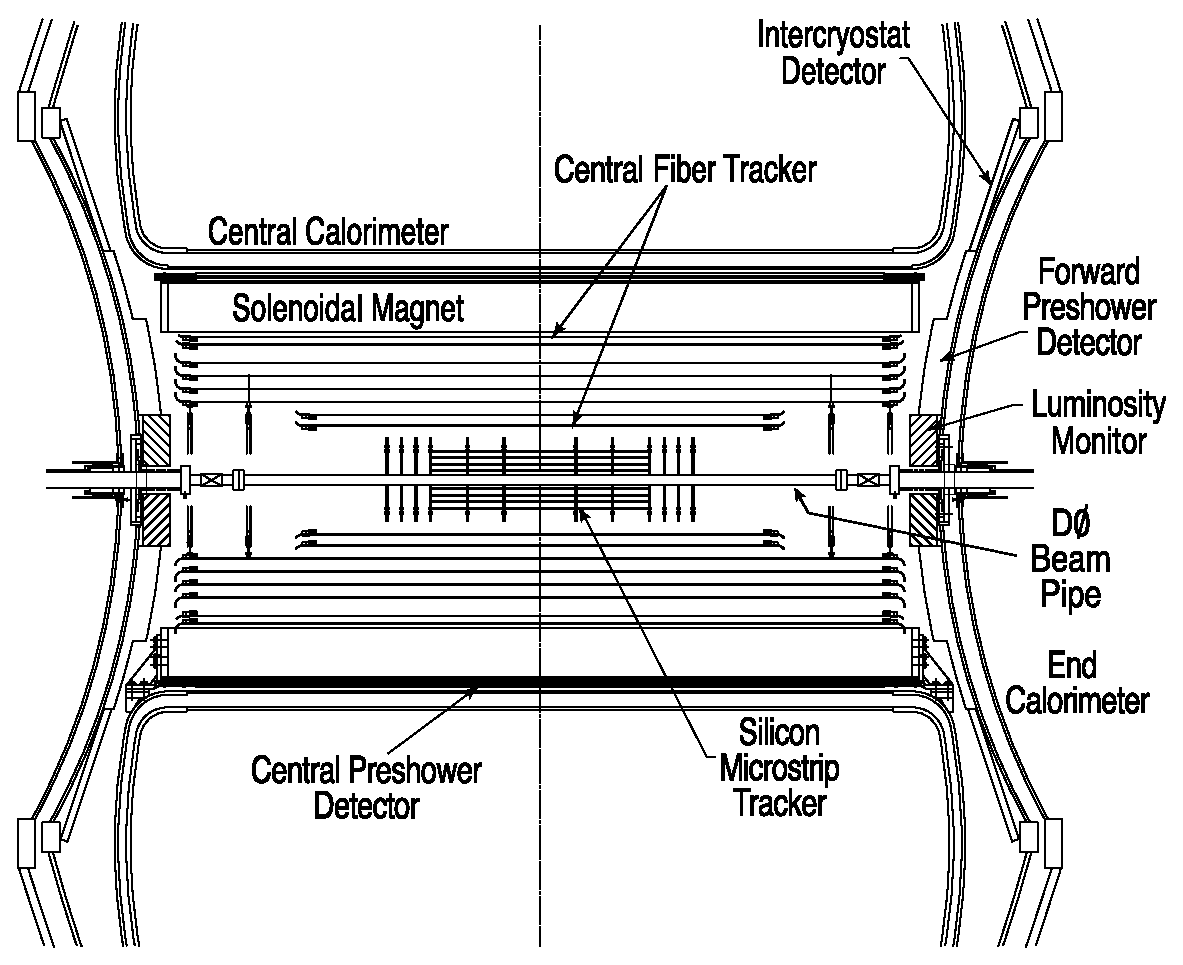
\includegraphics[width=0.75\textwidth]{eps/D0/InnerDetector.eps}
\end{center}
\vspace{-0.1in}
\caption{Schematic side-view of the three tracking detectors (SMT, CFT, and PS) as well as the superconducting solenoid magnet.}
\label{InnerDetector}
\end{figure}

\subsubsection{Silicon Microstrip Tracker}

The SMT is located immediately outside the Tevatron beam pipe, where the $\ppbar$~collisions take place, and provides high resolution position measurements of charged particles. The SMT is a collection of doped silicon detectors depleted of charged particles by the application of a reverse bias voltage. As a charged particle enters the depleted region it ionizes the silicon creating electron-hole pairs. The result of the applied electric field is to force the charges to drift towards active sensors. The typical drift distance for charges in the silicon is $300$~$\mu$m. The charge information is amplified and stored until a trigger accept is received (described in Section~\ref{triggersystem}) at which time the charge information is digitized and then stored in digital buffers until a second trigger accept is received. A schematic of the SMT is shown in Fig.~\ref{SMT}.

\begin{figure}[!h!tbp]
\begin{center}
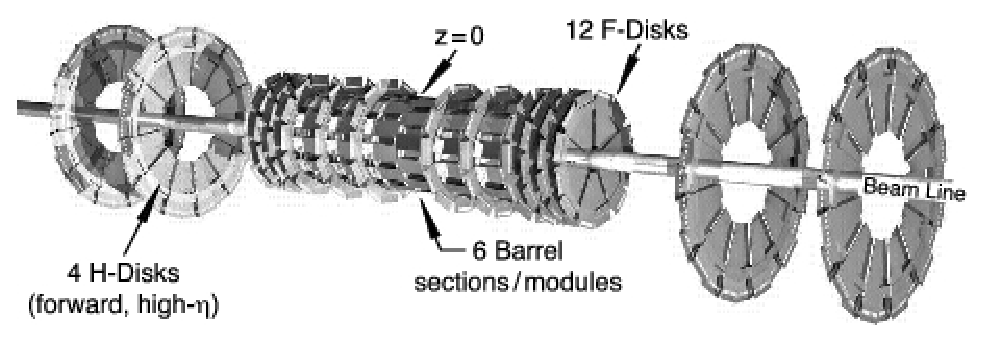
\includegraphics[width=0.75\textwidth]{eps/D0/SMT2.eps}
\end{center}
\vspace{-0.1in}
\caption{Schematic of the silicon microstrip tracker sub-detector.}
\label{SMT}
\end{figure}

The geometry of the SMT is dictated by the length of the interaction region~\footnote{Because the protons and antiprotons come in bunches, there is a relatively large distance along the $z$-axis where they can interact. The typical Gaussian width of the hard-scatter interactions is $25$~cm centered around z=0.} and a desire that each charged particle pass through as many layers of silicon as possible. The detector consists of three different structures to maximize the chance a charged particle with traverse the detector. The three structures are the barrel detectors, the F-discs, and the H-discs. The barrel detector is a set of six barrels concentric with the beam pipe that each contain four double-sided layers of silicon wafers. The barrels provide coverage for centrally produced charged particles with $|\eta|<1.1$. Layers 1 and 3 are oriented in a $90^{^\circ}$ stereo layout with respect to the beam pipe. Layers 2 and 4 are oriented in a $2^{^\circ}$ stereo layout. The F-discs are also double-sided silicon wafers. These silicon detectors are oriented perpendicular to the beam axis in contrast with the concentric barrels. There are twelve F-disks in the SMT, six in the central region that cap each barrel and six in the forward region. Each F-disk has 12 double-sided layers of silicon wafers. Finally, the SMT also has four silicon detectors at high $|z|$ called H-disks, which are also oriented perpendicular to the beam axis. Each H-disk contains 24 double-sided silicon wedges yielding 96 full "H-wedges" in total. In total the SMT has 912 individual readout modules and nearly 800,000 individual readout channels.


\subsubsection{Central Fiber Tracker}

Immediately outside of the SMT is the central fiber tracker (CFT) which occupies the radial space of 20 to 52 cm from the beam pipe. The CFT is organized into 8 layers of scintillating fibers which produce light when a charged particle traverses the fibers. Each layer of the CFT consists of two sets of fibers: one that is parallel with the beam axis and one that is rotated $3^{\circ}$ with respect to the beam axis. 
The fibers in the tracker are $835$~$\mu$m in diameter and composed of organic scintillating compounds surrounded by a thin layer of cladding designed to provide total internal reflection inside the fiber. The light produced in the fiber is carried out of the detector by wave guides with typical travel distances between 8 and 11 m. One end of each fiber is coated with sputtered aluminum which reflects 90$\%$ of the light back to the end which is read out. An endview schematic of the CFT layers and waveguides is shown in Fig.~\ref{CFT}.  Light produced in the CFT is recorded on silicon avalanche photon counters called VLPCs (visible light photon counter). The VLPCs operate at $9^{\circ}$~K to reduce thermal noise and achieve a quantum efficiency of $75\%$. 128 VLPCs are organized on one ``cassette", which is connected to the analog readout board.

\begin{figure}[!h!tbp]
\begin{center}
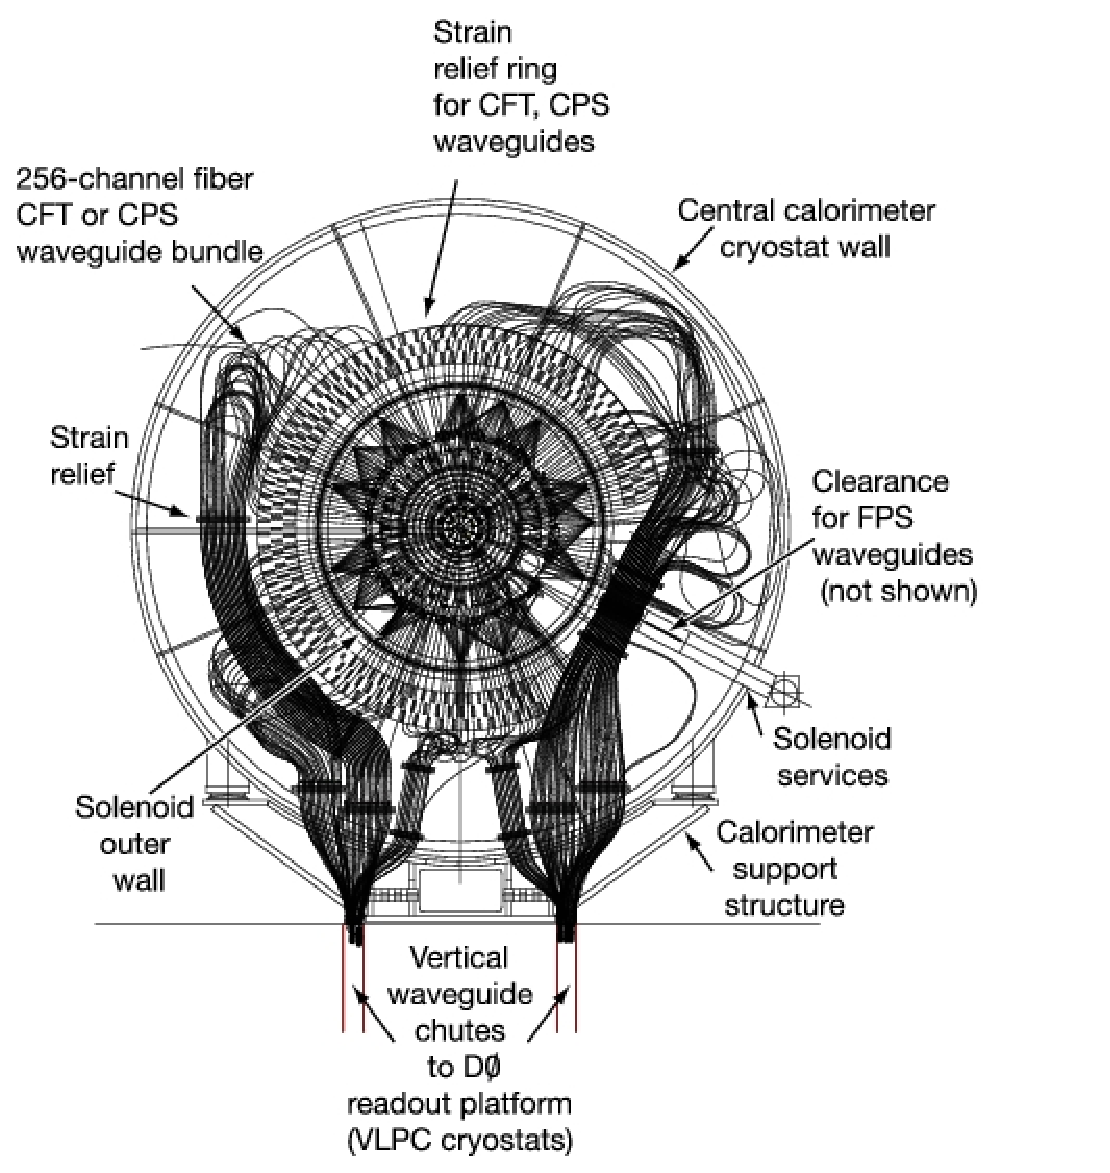
\includegraphics[width=0.75\textwidth]{eps/D0/CFT2.eps}
\end{center}
\vspace{-0.1in}
\caption{Schematic endview of the central fiber tracker with corresponding waveguides.}
\label{CFT}
\end{figure}


%\subsubsection{Preshower}


\subsection{Calorimetry}
\label{calorimetry}

The next layer of the $\dzero$~detector is the calorimeter. The calorimeter is designed to measure the energy of electromagnetically interacting particles such as electrons and photons as well as strongly interacting particles such as pions or neutrons. The $\dzero$~calorimeter is divided into three sub-detectors: one central region (CC) and two end-cap regions (EC) as seen in Fig.~\ref{Calorimeter}. Each region is encased in it's own cryostats held at a constant temperature of $90^{\circ}$~K. The region between the two cryostats, $0.8 < |\eta| < 1.4$, is called the inner cryostat region (ICR) and contains active scintillator to provide minimal energy measurement coverage in this region.

\begin{figure}[!h!tbp]
\begin{center}
\includegraphics[width=0.75\textwidth]{eps/D0/Calorimeter.eps}
\end{center}
\vspace{-0.1in}
\caption{3D view of the $\dzero$ calorimeter}
\label{Calorimeter}
\end{figure}

Each detector region, except the ICR, measures energy using a similar approach by inducing incoming particles to shower as they collide with a dense material. An example of an electromagnetic shower originating from a photon is shown in Fig.~\ref{EMshower}. As a particle from the created shower enters the active region it will ionize the active material, which is forced to move towards a sensor due to an applied bias voltage. The amount of charge collected on the sensor is then proportional to the energy deposited by the ionizing particle. The typical ion drift time is $\sim450$~ns.


\begin{figure}[!h!tbp]
\begin{center}
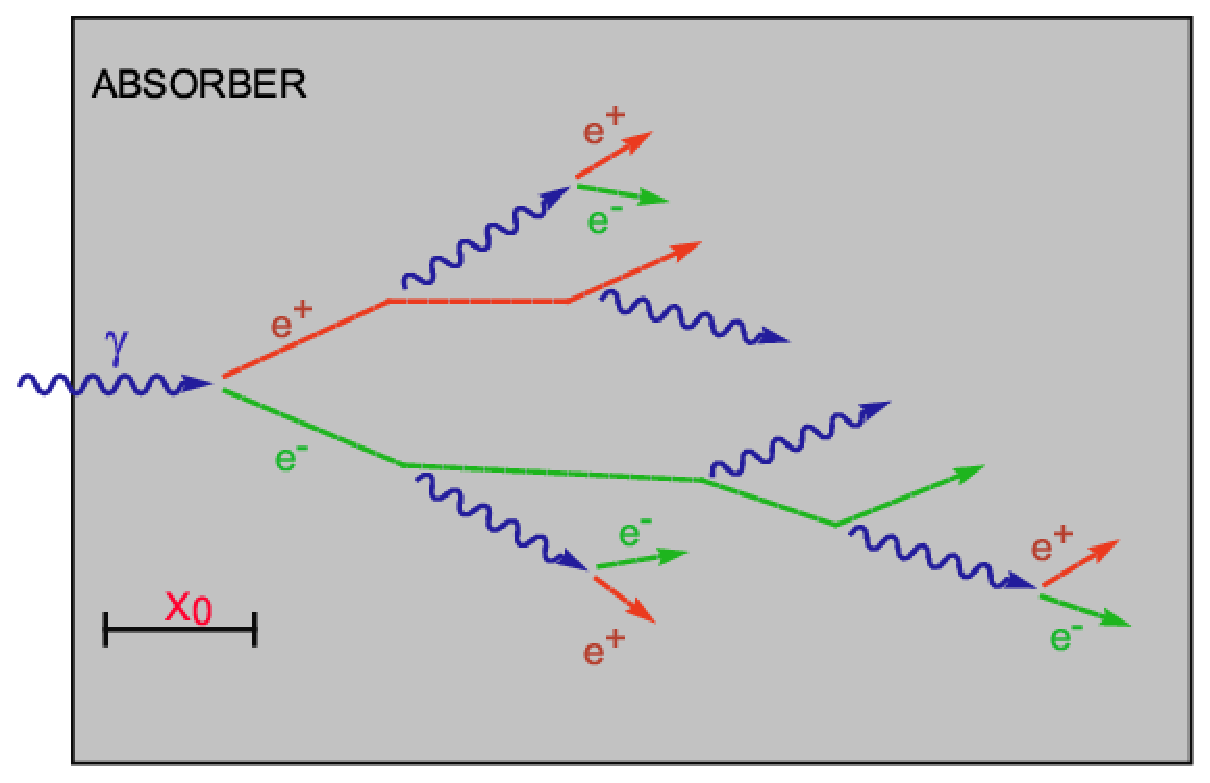
\includegraphics[width=0.75\textwidth]{eps/D0/shower.eps}
\end{center}
\vspace{-0.1in}
\caption{Initial stages of an electromagnetic shower caused by a photon interacting with an absorber material. The radiation length, $x_{0}$, is the typical distance a photon will travel before producing an $e^{+}e^{-}$ pair or a distance before an electron will radiate a photon.}
\label{EMshower}
\end{figure}

The $\dzero$ calorimeter consists of an inner detector called the EM calorimeter and an outer detector called the hadronic calorimeter. The EM calorimeter is constructed of alternating layers of depleted Uranium, which acts as the shower inducing material or absorber, and liquid Argon, which acts as the active medium. The depleted Uranium plates are 3-mm thick in the central region and 4 mm thick in the forward end-cap region while the liquid Argon active region is 2.3 mm thick. An cartoon drawing of this arrangement can been seen in Fig.~\ref{CalorimeterCell}. The EM calorimeter has four layers of cells which represent nearly 21 radiation lengths for incoming particles. The hadronic calorimeter is actually two detectors: one called the fine hadronic calorimeter which employs 6 mm thick Ur-Ni alloy as the absorber material and the coarse hadronic calorimeter which uses 46.5 mm thick plates of copper in the central region and stainless steel in the forward region. The hadronic calorimeter also uses liquid Argon as the active material similar to the EM calorimeter. The combination of the fine and coarse hadronic calorimeters provides an additional 7 radiation lengths to the detector. The numerous radiation lengths are important to ensure that an object deposits nearly all of it's energy in the detector as well as providing shielding for the muon detector described in Section~\ref{muondetector}.


\begin{figure}[!h!tbp]
\begin{center}
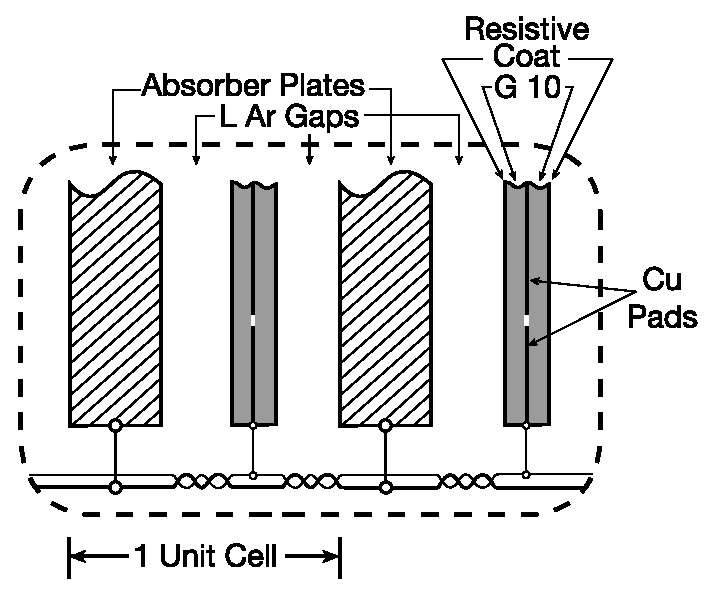
\includegraphics[width=0.75\textwidth]{eps/D0/CalorimeterCell.eps}
\end{center}
\vspace{-0.1in}
\caption{Example of typical calorimeter cell of alternating absorber and active material. Particles traverse the calorimeter cell from left to right in this diagram.}
\label{CalorimeterCell}
\end{figure}

The $\dzero$~calorimeter also has fine segmentation which allows for a finer energy measurement of particles as they shower in the detector. The segmentation of the EM calorimeter in $\delta\eta \times \delta\phi$ is $0.1 \times 0.1$ for all layers except the third layer, where the segmentation is $0.05 \times 0.05$. The finer segmentation in the third layer is because the electromagnetic shower is expected to reach a maximum in this layer. The fine hadronic layers of the calorimeter also have a segmentation in $\delta\eta \times \delta\phi$ of $0.1 \times 0.1$, while the segmentation in the coarse hadronic calorimeter is $0.2 \times 0.2$. An octant of the $\dzero$~calorimeters including segmentation can be seen in Fig.~\ref{CalorimeterSegmentation}. 

\begin{figure}[!h!tbp]
\begin{center}
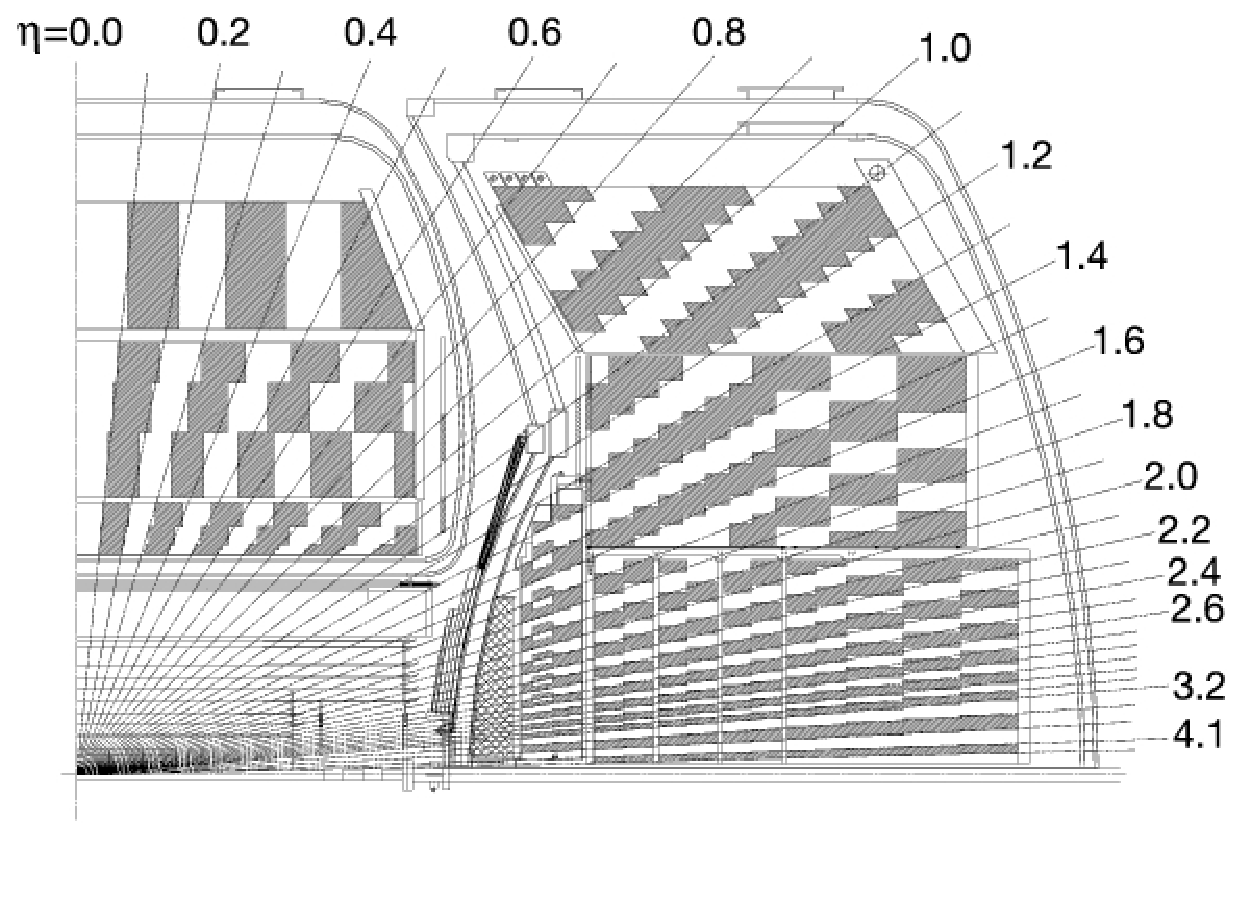
\includegraphics[width=0.75\textwidth]{eps/D0/CalorimeterSegmentation2.eps}
\end{center}
\vspace{-0.1in}
\caption{Octant of the $\dzero$~calorimeter. The fine segmentation of the calorimeter can be clearly seen in this diagram.}
\label{CalorimeterSegmentation}
\end{figure}



\subsection{Luminosity Monitor}
\label{luminositydetector}

Located directly in front of the end-cap calorimeters, covering a $\eta$ range between 2.7 and 4.4, is the luminosity monitor, which collects information about inelastic $\ppbar$~collisions for each bunch crossing. The luminosity monitor is a set of 24 plastic scintillators which can detect low angle (high $\eta$) fragments from the break-up of the protons in the $\ppbar$~collision. The scintillators produce light when the charged fragments traverse the detector and that light is recorded by photo-multiplier tubes. A schematic of the luminosity monitor is shown in Fig.~\ref{Luminosity}.

\begin{figure}[!h!tbp]
\begin{center}
\includegraphics[width=0.75\textwidth]{eps/D0/Luminosity.eps}
\end{center}
\vspace{-0.1in}
\caption{Schematic of the $\dzero$ luminosity monitor shown in relation to the beam pipe, SMT, and endcap calorimeter.}
\label{Luminosity}
\end{figure}


Collecting information about inelastic collisions is vital to properly normalize all data collected at $\dzero$. The luminosity monitor is designed to measure the inelastic $\ppbar$~cross section, which is a quantity that is known from measurements by previous experiments. By measuring the inelastic $\ppbar$~cross section the total integrated luminosity to which the $\dzero$~detector has been exposed to can be measured. A derivation of the luminosity from the measured $\ppbar$~inelastic cross section can be found in Appendix~\ref{lumi}.

Along with providing a luminosity measurement, the detector also acts a fast vertex finder. By measuring the relative difference of coincidence counts in the North and South detectors, the $z$ position of the vertex can be determined from Eq.~\ref{zpos}, where $t_{\pm}$ are the time measured by the North (+) and South (-) detectors, respectively. The time of flight resolution for the luminosity detector is 0.3 ns.

\begin{equation}
\label{zpos}
z = \frac{c}{2}(t_{-} - t_{+})
\end{equation}

\subsection{Muon Detector}
\label{muondetector}

The outer-most layer of the $\dzero$~detector is the muon system. A special detector is required to measure muons because they do not deposit much energy in the tracker or calorimeter and thus a confirmation of their presence using these sub-detectors alone is difficult to infer. The muon detector has two active regions called the central region for $|\eta|<1$ and the forward region $1<|\eta|<2$. The system also employs a 2 T toroid iron magnet to bend the muons from their original paths. The addition of the magnetic field helps to provide a local momentum measurement in the event the momentum can not be determined from the tracking detector. Additional shielding surrounding the beam pipe near the forward muon detector is designed to reduce spurious beam effects which dramatically reduces the amount of radiation to which to detector is exposed. A schematic of the muon system and the beam shielding can be seen in Fig.~\ref{MuonDetector}.

\begin{figure}[!h!tbp]
\begin{center}
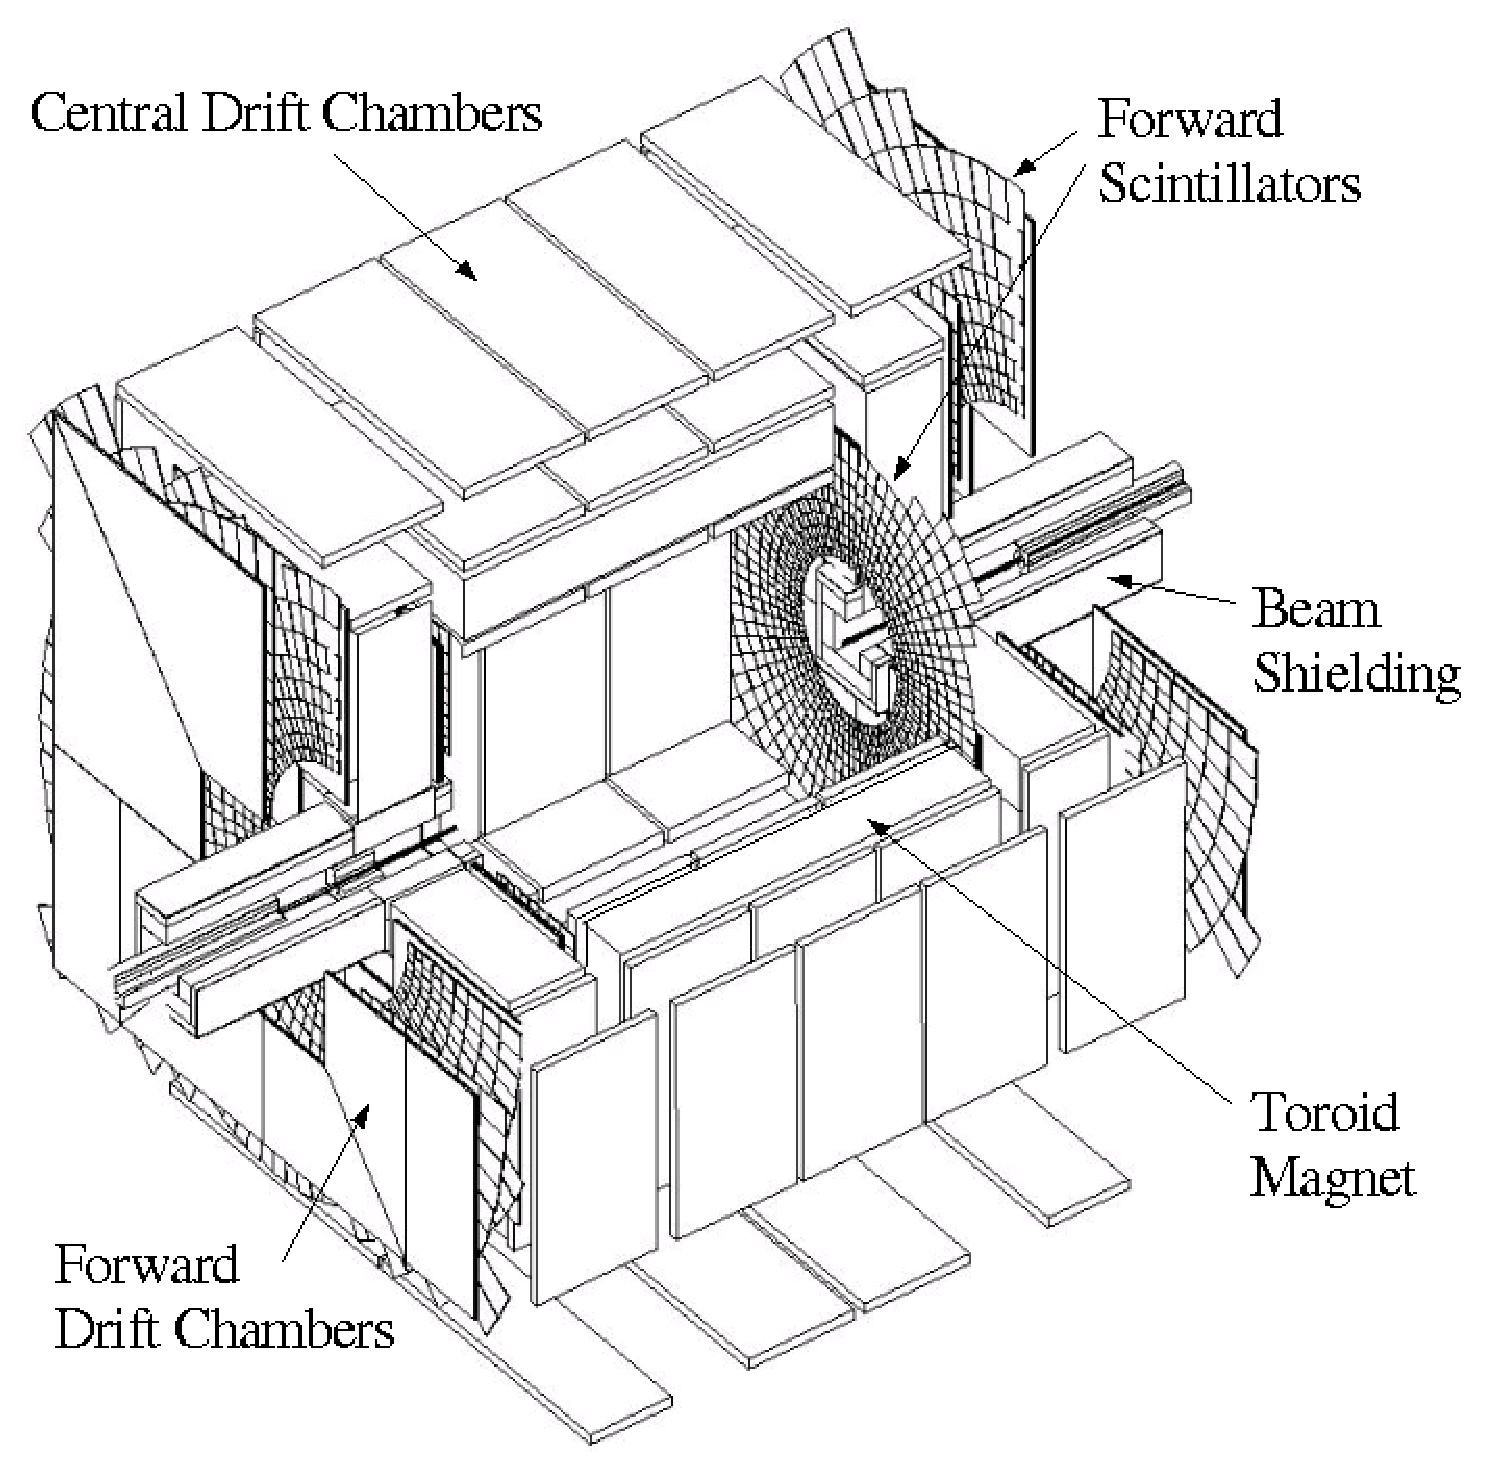
\includegraphics[width=0.75\textwidth]{eps/D0/mudet.eps}
\end{center}
\vspace{-0.1in}
\caption{3D view of the $\dzero$ muon detector.}
\label{MuonDetector}
\end{figure}

The muon system at $\dzero$ is a three layer detector, both in the central and forward regions, consisting of drift chambers for precise position measurement and scintillator counters for muon identification and position measurements. The scintillator counters produce light when the muon passes through the detector which is then collected by a photo-multiplier tube. The drift chambers have a central wire held at a large voltage surrounded by an inert gas. As the muon enters the chamber it will ionize the gaseous organic compound mixture and the resulting free charges will begin to drift towards the wire. The position of the muon is found by measuring the current profile in time of the charges as they collect on the wire. In the central region, the drift chambers are called PDTs (proportional drift tubes) and rather are large with typical areas of 2.8 $\times$ 5.6 m$^{2}$. The forward region uses smaller drift chambers called MDTs (mimi drift tubes), which are a collection of eight cells of size 9.4 $\times$ 9.4 mm$^{2}$. The position resolution of the drift chambers is $\sim$1 mm.

\subsection{Trigger System}
\label{triggersystem}

The previous sections in this chapter describe how the $\dzero$~detector collects information from $\ppbar$~collisions at the Tevatron, which occur every $396$~ns. While $\dzero$ records information about every collision, it does not save every event to tape for two reasons: most collisions at the Tevatron are small angle inelastic collisions which have already been well studied and the total rate of data one can reliably store to tape is limited to $\sim$30MB/s. Because $\dzero$~can not save every event, a sophisticated trigger system is employed to reduce the total rate to tape to $50$~Hz. This trigger system attempts to select the most "interesting" events, which will be used for an analysis or future calibration of the detector.

The trigger system is comprised of three independent stages called level1 (L1), level2 (L2), and level3 (L3), which reduces the total event from $1.7$~MHz to $50$~Hz. A schematic of the combined trigger system is shown in Fig.~\ref{Trigger}. The L1 system is composed of hardware trigger elements and has the goal of reducing the initial rate of  $1.7$~MHz to $1.5$~kHz. Because the L1 trigger must act quickly to either accept or reject an event, the tools available for selecting interesting events is limited. At L1 only calorimeter trigger towers, which are layers of calorimter cell energies within a $\delta\eta \times \delta\phi = 0.2 \times 0.2$ space, signals in the muon drift chambers or scintillators, and the transverse momentum of charged particle tracks in the central fiber tracker are available for trigger decisions. The L1 system allows $3.5~\mu$s for a decision to be made. Events which take longer to process are rejected.

\begin{figure}[!h!tbp]
\begin{center}
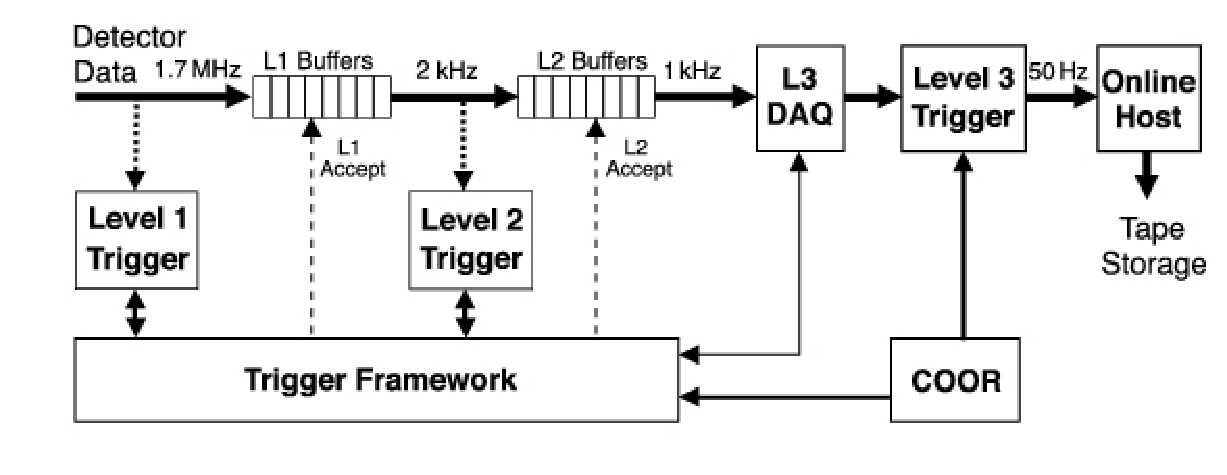
\includegraphics[width=0.75\textwidth]{eps/D0/TriggerFlow2.eps}
\end{center}
\vspace{-0.1in}
\caption{Cartoon drawing of the $\dzero$ trigger system.}
\label{Trigger}
\end{figure}

The L2 trigger acts on all events which pass the L1 trigger and is designed to reduce the rate from 1.5kHz to $700$Hz. The L2 trigger uses detector specific pre-processing boards and a global detector board to make trigger decisions. The pre-processors collect data from the L1 trigger system as well as readout information from the individual detectors. The pre-processors use this information to form physics objects such as electrons, jets, and missing E$_{T}$~\footnote{Physics objects and event-wide kinematic variables such as missing E$_{T}$~are fully described in Chapter~\ref{EventSelection}.}. A global L2 pre-processor uses all the information from the sub-detector pre-processors to make trigger make decisions based on event-wide kinematics.

After a L2 trigger accept, the information from each sub detector is collected and stored in memory on a single board computer (SBC) located in the detector readout crate. The information from the readout crate routed to one of many computers used to form a L3 trigger decision. The L3 trigger attempts to reconstruct the event and uses event-wide as well as single object kinematics. If the event satistfies the criteria of the L3 trigger the event is recorded and stored on tape. A more complete description of the L3 trigger and data acquisition system is given in Appendix~\ref{Level3}.
